\chapter{Реализация и экспериментальная проверка}

Coq — интерактивное программное средство доказательства
теорем, использующее собственный язык функционального
программирования с зависимыми типами. Позволяет записывать
математические теоремы и их доказательства, удобно модифицировать
их, проверяет их на правильность. Пользователь интерактивно создаёт
доказательство сверху вниз, начиная с цели (то есть от гипотезы,
которую необходимо доказать). Coq может автоматически находить
доказательства в некоторых ограниченных теориях с помощью так
называемых тактик. Coq применяется для верификации программ\cite{huet}.

Формальная спецификация в Gallina состоит из последовательности объявлений (
declarations) и определений (definitions). Также можно вводить комманды, но
они не являются частью формальной спецификации, а выполняют информационные 
запросы или сервисные функции\cite{huet}. 

\section{Реализация CIC в системе автоматического доказательства Coq}
Формальной основой Coq, как уже было отмечено ранее является индуктивное 
исчисление конструкций (CIC). Выражения в CIC  это термы, а все термы имеют 
типы, существуют типы для функций (или программ), атомик-типы --- типы 
данных, типы для доказательств, а так же типы для типов.  В частности, любой 
объект, обрабатываемый формализмом, должен принадлежать типу. Например, 
квантор всеобщности относится к типу. Типы для типов называются сортами. Типы 
и сорта сами по себе являются термами.

У всех сортов есть тип и существует бесконечная валидная иерархия типизации, 
чьи базовые сорта - Prop и Set.
Сорт Prop намеревается быть типом логических предложений. Если M - логическое 
предложение, то он обозначает класс членов, представляющих доказательства M. 
Объект m, принадлежащий M, свидетельствует о том, что M доказуемо. Объектом 
типа Prop называется предложение.
Сорт Set представляет собой тип небольших наборов. Это включает в себя типы 
данных, такие как логические, числовые, а также продукции, подмножества и 
типы функций по этим типам данных.
Сортами Prop и Set можно манипулировать как обычными термами, а это значит 
что они сами имеют тип. Поскольку предположение что сорт Set имеет тип Set 
приводит к инконсистентности теории \cite{coquand1986analysis}, язык CIC 
имеет бесконечно много сортов. В дополнение к Set and Prop имеется иерархия 
юниверсов Type(i) для любого целого i.

Как и Set Type(i) содержат маленькие множества, такие как логический тип, 
натуральные числа, а также подмножества и типы функций . Но, в отличие от 
Set, они также содержат большие множества --- сорта Set и Type(j) для j <i, а 
также все продукции, подмножества и типы функций над этими сортами.

Формально множество сортов S определяется следующим образом:
$S \ \equiv \ {Prop, \ Set, \ Type(i) \ | \ i \in N} $


$Prop:Type(1), \ Set:Type(1), \ and Type(i):Type(i+1)$


Пользователь не должен явно указывать индекс i при обращении к типу юниверса (
i). Он только пишет Type. Сама система генерирует для каждого экземпляра Type 
новый индекс для юниверса и проверяет, что ограничения между этими индексами 
могут быть решены. С точки зрения пользователя имеется Type: Type.

\section{Спецификация языка Gallina}

Теории строятся из аксиом, гипотез, параметров, лемм, теорем и определений 
констант, функций, предикатов и множеств. Язык Gallina позволяет 
разрабатывать математические теории и доказательства спецификаций программ.

Квалифицированные идентификаторы (qualid) обозначают глобальные константы (
определения, леммы, теоремы, замечания или факты), глобальные переменные (
параметры или аксиомы), индуктивные типы или конструкторы индуктивных типов. 
Простые идентификаторы (или короткий идентификатор) являются синтаксическим 
подмножеством квалифицированных идентификаторов. Идентификаторы также могут 
обозначать локальные переменные, какие нет у квалифицированных идентификаторов.

Числа не имеют определенной семантики в исчислении. Это простые обозначения, 
которые могут быть привязаны к объектам через механизм обозначения. 
Первоначально цифры связаны с представлением Пеано натуральных
чисел.

Различные конструкции, такие как fun, forall, fix и cofix связывают переменные.
Связывание представляется при помощи идентификатора. Если переменная привязки 
не используется в выражении, идентификатор может быть заменен символом _. 
Когда тип связанной переменной не может быть синтезирован системой, ее можно 
указать с помощью обозначения $(ident: \ type)$. Существует также обозначение 
последовательности переменных привязки, имеющих один и тот же тип: $(ident_{1} \ \ldots \  ident_{n}: \ type)$. Некоторые конструкции позволяют привязывать 
переменную к значению. Это называется <<let-binder>>. В let-binder 
одновременно может быть введена только одна переменная. Также можно указать 
тип переменной следующим образом: $(ident: \ term: \ = \ term)$.
Возможны списки binder-ов. В случае fun и forall предполагаетя что хотя бы 
одно из связываний является предположением, иначе они становятся идентичными.

Выражение $fun \ ident: \ type \ => \ term$ определяет абстракцию переменной 
ident, типа type, над термом term. Выражение $forall \ ident: \ type, \ term$ 
обозначает произведение переменной ident типа type, над термом term. 
Выражение $term_{0} \ term_{1}$ обозначает применение $term_{0}$ к $term_{1}$.
Выражение $term: \ type$ является выражением приведения типа. Выражение $let 
\ ident \ := \ term_{1} \ in \ term_{2}$ локально связывает $term_{1}$ с 
переменной  $ident$ в терме $term_{2}$.
  
	
\section{Механизм вывода}

Имеется параллель между интуиционистской импликацией и квантором
всеобщности, с одной стороны, и функциональным типом и зависимым
произведением параметрического семейства типов, с другой.
Это соответствие приводит к интерпретации интуиционистской логики в
теории зависимых типов: высказывания интерпретируются типами (все-
ми или некоторыми), а предикаты --- семействами типов, зависящими от
параметров. Верность высказывания означает населенность (непустоту)
соответствующего типа. Классическая логика эмулируется дополнитель-
ным контекстом, который обеспечивает непустоту типа, соответствующе-
го закону исключенного третьего\cite{msu}.

В рамках указанной парадигмы обоснование справедливости (верности) 
высказывания A означает предъявление объекта типа A. В теории типов объектами 
служат типизованные $\lambda$-термы. Именно они и играют роль доказательств 
соответствующих высказываний. Их также можно рассматривать как строчные 
записи деревьев вывода, доказывающих эти высказывания в формализме 
натурального вывода. Задача проверки правильности типизации термов для 
практически применяемых вариантов теории типов разрешима за разумное время, 
что позволяет автоматически верифицировать соответствующие доказательства. 
Непосредственное выписывание подходящих $\lambda$-термов оказывается 
практически невозможным ввиду их размера и сложности. Система Coq (и другие 
аналогичные интерактивные системы построения доказательств) упрощают эту 
задачу, позволяя строить соответствующие термы интерактивно, с привлечением 
ряда алгоритмов поиска выводов, частично автоматизирующих процесс построения \cite{msu}.


Формализм теории типов оперирует с секвенциями вида

$x_{1}:A_{1}, \ x_{2}:A_{2}(x_{1}), \  \ldots \ , \  x_{n}:A_{n}(x_{1}, \ 
\ldots \ , \ x_{n−1}) \ \vdash \  t(x_{1}, \ \ldots \ , \ x_{n}):B(x_{1}, \ 
\ldots \ , \ x_{n}$),
формализующими суждения о типизации <<если $x_{1}$ имеет тип $A_{1}$, $x_{2}$ 
имеет тип $A_{2}(x_{1})$,$\ldots$ , то $t(x_{1}, \ldots , x_{n})$ имеет тип $B
(x_{1}, \ldots , x_{n})$>>.

Работа пользователя в системе Coq направлена на построение соответствующего 
терма $t(x_{1}, \ldots , x_{n})$. Доступная ему информация описывается 
секвенцией $x_{1}:A_{1}, x_{2}:A_{2}(x_{1}), \ldots , x_{n}:A_{n}(x_{1},\ldots
 , x_{n−1}) \vdash (???) :B(x_{1}, \ldots , x_{n})$ с метапеременной (???), 
значение которой надо определить.

\begin{figure}[h,t]
	\centering
		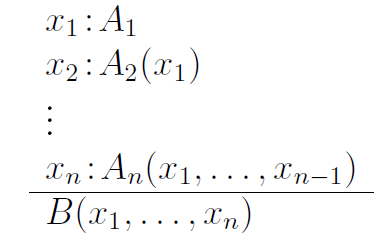
\includegraphics[width=0.30\textwidth]{img/dsdjl.png}
	\caption{l}
	\label{fig:dsdjl}
\end{figure}


Один шаг интерактивного построения доказательства состоит в том, что 
пользователь выбирает одну из имеющихся тактик, а система ее применяет. 
Многие тактики для своего применения требуют дополнительные параметры, 
которые также указываются пользователем. Тактика представляет собой сведение 
решаемой задачи построения терма $t$, для которого секвенция (цель) $\Gamma 
\vdash t : A$ выводима (в CIC), к аналогичным задачам для некоторых других 
секвенций (подцелей) $\Gamma_{1} \vdash t_{1} : A_{1}, \ldots ,\Gamma_{k} 
\vdash t_{k} : A_{k}, k \geq 0$. Тактики соответствуют допустимым правилам 
исчисления CIC, а также содержат алгоритмы построения искомого терма $t$ по 
термам $t_{1}, \ldots, t_{k}$. При применении тактики изображающая задачу 
таблица (без t) $\frac{\Gamma}{A}$ превращается в $\frac{\Gamma_{1}}{A_{1}}  
\ldots \frac{\Gamma_{k}}{A_{k}}$.
Аналогичные шаги применяются к подцелям и т.д., пока количество
подцелей не сократится до 0. Система запоминает последовательность
примененных тактик и восстанавливает искомый терм $t$ c помощью 
соответствующих алгоритмов. При этом система постоянно контролирует 
правильность типизации всех термов, что исключает возможность получения 
ошибочных доказательств\cite{msu}. В системе автоматического доказательства 
Coq существует возможность самостоятельно писать тактики используя специально 
разработанный для этого язык разработки тактик.

\begin{figure}[ht]
	\centering
		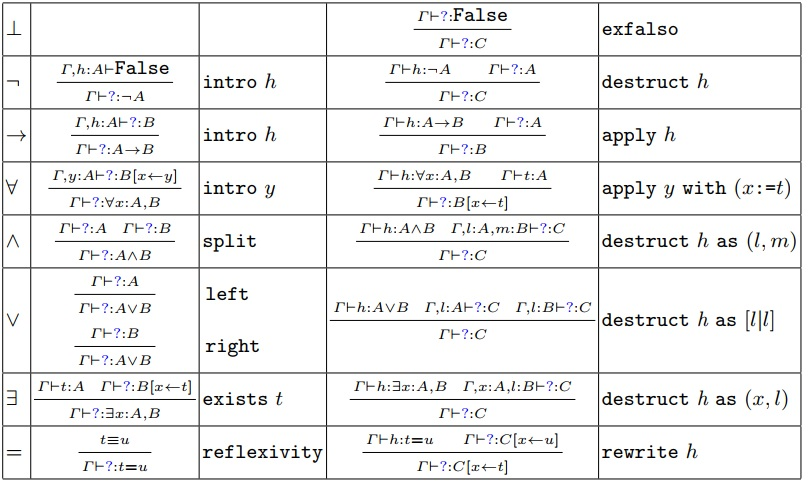
\includegraphics[width=0.90\textwidth]{img/тактики.jpg}
	\caption{Логические правила и соответствующие им тактики}
	\label{fig:тактики}
\end{figure}

В большинстве случаев, для построения доказательства в системе Coq 
используется такой подход как <<целенапрвленное доказательство>> (\textit{goal 
directed proof}) который использует следующий тип сценария\cite{bertot}:
\begin{enumerate}
	\item Пользователь вводит утверждение, которое он хочет доказать, используя 
команду Theorem или Lemma, при этом именуя ее.
\item Система Coq отображает формулу в качестве формулы, которая должна быть 
доказана, возможно, предоставляя контекст локальных фактов, которые могут 
быть использованы для этого доказательства (контекст отображается над 
горизонтальной линией, написанной =====, цель отображается под горизонтальной 
линия).
\item Пользователь вводит команду(тактики) для декомпозиции цели на более 
простые подцели.
\item Система Coq отображает список формул, которые еще нужно доказать.
\item Повторяется 3 шаг до тех пор, пока не останется ни одной формулы, 
которую нужно доказать.
\end{enumerate}

Когда нет больше целей, доказательство завершено, оно сохраняется при помощи 
команды Qed с именем заданным на 1 шаге.
Оформляется теорема следующим образом:

\begin{verbatim}
Theorem <идентификатор>: < формулировка>.
Proof.
	<доказательство>
Qed.
\end{verbatim}

В дальнейшем <идентификатор> можно использовать как любую другую константу 
указанного типа. Тем самым Theorem представляет собой вариант интерактивного 
определения констант\cite{bertot}.

\section{Введение констант}

Описание прикладных теорий в системе Coq сводится к введению новых
имен (констант). Это аппарат позволяет единообразно описывать как
язык, так и аксиоматику теории. Для того, чтобы постулировать некоторое 
утверждение, достаточно формализовать его в виде типа $A:Prop$,
после чего декларировать непустоту типа A введением новой (свободной)
константы c:A. Механизм секций позволяет объединить основные определения и 
теоремы теории в единое целое\cite{msu}.

Ключевые слова $Variable$ и $Hypothesis$ (а также $Variables$, $Parameter$,
$Parameters$, $Axiom$, $Conjecture$) являются почти синонимами. Они позволяют 
ввести в контекст новые константы (имена) и объявить их типы\cite{bertot}.

Некоторое различие между группами ($Variable$, $Variables$, $Parameter$,
$Parameters$) и ($Hypothesis$, $Axiom$, $Conjecture$) проявляется лишь при
использовании механизма секций. 
\begin{verbatim}
Section <название секции>.
...
End <название секции>.
\end{verbatim}
Это окружение позволяет ограничить пределами секции область действия 
деклараций констант, введенных внутри секции с помощью ключевых слов 
$Variable$, $Variables$, $Parameter$, $Parameters$. Вне секции эти константы 
недоступны. Там они преобразуются в дополнительные параметры всех 
определенных внутри секции имен.

Введенные с помощью декларации имена являются свободными константами --- им 
нельзя присвоить какие-нибудь значения, отличные от них самих. Для 
определения новых имен через уже имеющиеся служит конструкция Definition\cite{bertot}.

Более сложный вариант определений --- индуктивное определение типа ---
вводится ключевым словом Inductive. В основе лежит семантика наименьшей 
неподвижной точки. Задаются конструкторы объектов определяемого типа, а сам 
тип представляет собой наименьшее множество, замкнутое относительно 
применения конструкторов\cite{bertot}.

\section{Разбор случаев}
Пусть задано индуктивное определение типа $T$ с конструкторами $c_{1}, \ldots 
, c_{k}$, где $c_{i}$ представляет функцию от $n_{i}$ аргументов со 
значениями в типе $T$. Каждый терм $t$ типа $T$ имеет вид $c_{i}t_{i,1} \ldots t_{i,n_{i}}$ для 
некоторого $i$, причем это представление единственно. Разбор случаев позволяет через $t$ определить 
выражение $h(t)$ разными способами в зависимости от вида терма t\cite{msu}:

\[ h(t) =
  \begin{cases}
    h_{1}(t_{1,1}  \ldots t_{1,n_{1}}),     & если t = c_{1}t_{1,1}  \ldots t_{1,n_{1}}\\
		\ldots \\
     h_{k}(t_{k,1}  \ldots t_{k,n_{k}}),     & если t = c_{k}t_{k,1}  \ldots t_{k,n_{k}}
  \end{cases}
\]

Чтобы выражению $h(t)$ удалось приписать тип, достаточно потребовать,
чтобы все термы $h_{i}(t_{i,1} \ldots t_{i,n_{i}})$ имели общий тип T_{1}. Теория зависимых
типов позволяет ослабить это условие: достаточно иметь семейство типов
$T_{1}(z)$, индексированное элементами $z :T$, и требовать, чтобы
$h_{i}(t_{i,1} \ldots t_{i,n_{i}}) :T_{1}(t)$ при $t = c_{i}t_{i,1} \ldots t_{i,n_{i}}$ .
Соответствующая редукция  заменяет терм $h(t)$ на $h_{i}(t_{i,1} \ldots t_{i,n_{i}})$,
сохраняя его тип $T_{1}(t)$.

В синтаксисе языка Gallina системы Coq разбор случаев реализует конструкция match:
\begin{verbatim}
match term [dep_ret_type] with
| C1 _ … _ => term1
.......
| Cn _ … _ => termn
end.
\end{verbatim}